\chapter{Cover path planning problem } 


\minitoc




   \subsubsection{Sorted waypoints and path planning} \label{sorted_}
In the previous section, the method to obtain the list of waypoints has been detailed. The list of waypoints needs now to be sorted to compute an efficient path with smoother shape and shorter travelling distance. 


There are several ways to formulate this problem. In this paper, two methods have been implemented and compared.
\subsubsection*{a)}{Shortest Path Problem}
\\Normally, finding a shortest path between two points in configuration space is mature enough. In our case we assume the waypoints as multi goals. So the planning in this method will simply finding at every waypoint the shortest Euclidean distance from the other available non-traversed waypoints. Based on that a ranked waypoints list will be generated. This will not guarantee a globally shortest distance, but will only choose the shortest distance every time a waypoint is visited.

%The first way is to assume the waypoints as multi goals. So the plannig in this method will simply finding at every waypoint the shortest euclidean distance to the other waypoints. Based on that a ranked waypoints list will be generated. 

\subsubsection*{Traveling Sales Man Problem)}

%\begin{figure}[t]
%  \centering
% %  \subfigure[Poses of every image captured in the room]{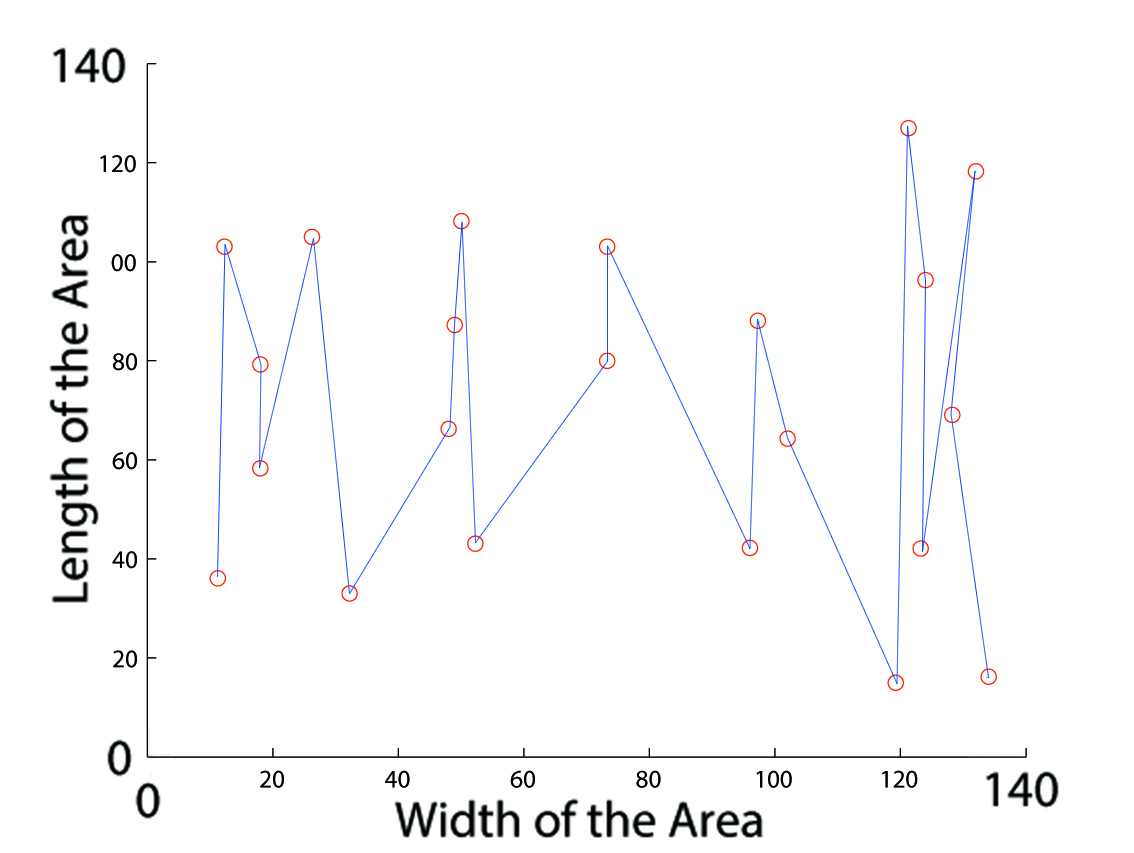
\includegraphics[width=0.85\textwidth]{img/22pts_WaypointsDijktra2.jpg}}
%   \hfill
% %  \subfigure[Path compute with Dijktra multi goal]{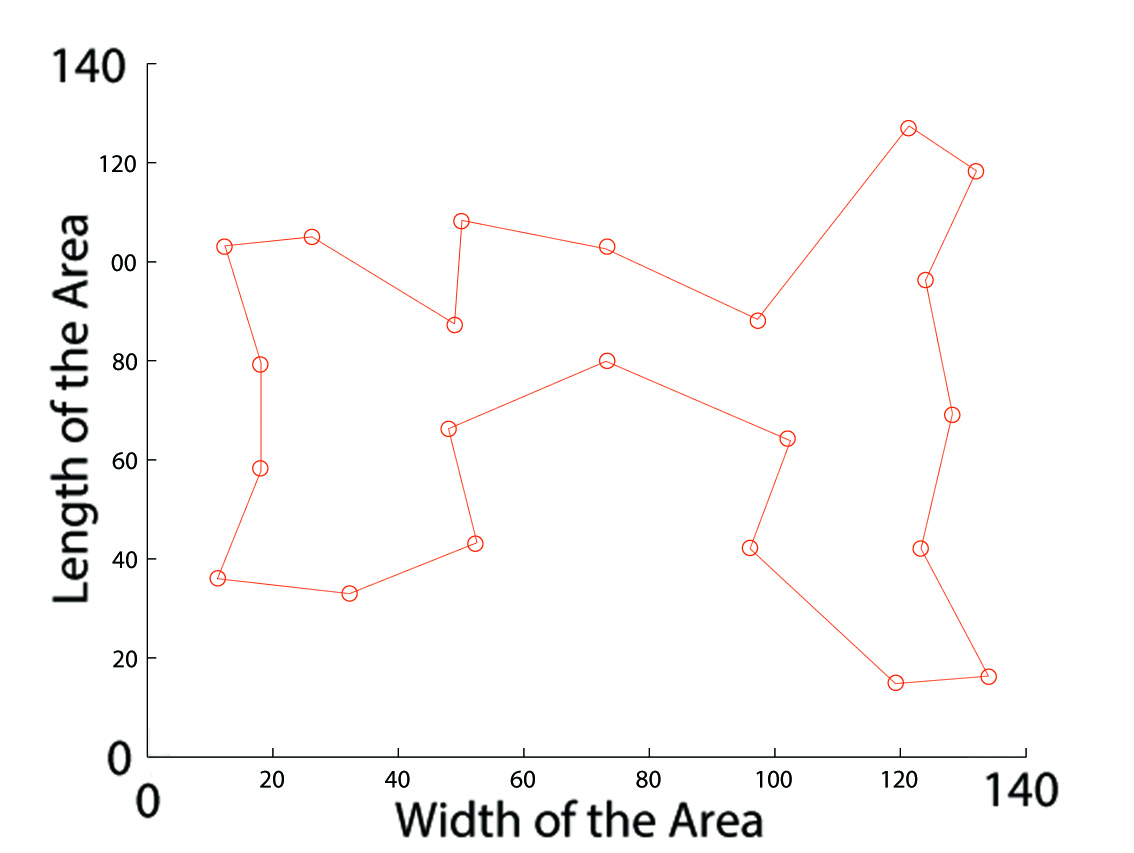
\includegraphics[width=0.85\textwidth]{img/22pts_WaypointsGA2.jpg}}
%  \caption{optimisation of the path plannig}\label{fig:Path_planning} 
%\end{figure}

 \begin{mfigures}[!]{optimisation of the path plannig}{fig:Path_planning} \centering
\mfigure{width=.4\linewidth}{img/22pts_WaypointsDijktra2.jpg}{Poses of every image captured in the room.}{subfig:Dijktra}
\hspace{1cm}
\mfigure{width=.4\linewidth}{img/22pts_WaypointsGA2.jpg}{Path compute with Dijktra multi goal.}{subfig:GATSP}
\end{mfigures} 

The sorted path can be formulated as travelling salesman optimization problem  
(TSP).
%with minimum distance as the cost function
Every node which is a point in space is represented as a city and the Euclidean distances between the cities are calculated and used as a cost function. The path is organized based on the minimum distance traversing over all the cities (or waypoints). To find an optimized solution GA is here again used.

The privilege of TSP problem formulation and solving it using GA over the other shortest path algorithms like Dijkstra, is that it provides global  complete solution traversing all the waypoints not finding a path from a starting node  to a goal node. The GA approach is more clarified and discussed by Trevor \textit{et al}.\cite{GA_Path}. 


The distance covered by a path that is planned by GA is 513 meters, which is shorter by the factor of 1.8 compared to the distance covered by Dijsktra multi goal approach which is 963 meters. Using the GA  to optimize  the scheduling problem of waypoint makes a more efficient result and especially the GA unlike the Dijsktra multi goal, it is more efficient to sort a high number of waypoints.\\ 








\section{Splitting the problem }
	Splitting the problem 
			\subsection{Positioning of the waypoint }
			
			\subsection{Number of waypoint }
				\subsubsection{Fix number of waypoints}
				intro  and prerequi to  the estimate the number of waypoints.
				\subsubsection{Estimate the number of waypoints}
Is difficult to estimate properly the minimum of waypoints are necessary to cover a complex area.
To do so, a two-step procedure has been implemented which rest on the pose optimization of a fixed number of cameras or waypoints introduce in the precedent section. 
The first step is to find the minimum number of waypoints depending on the area to cover like formulated in the
 Eq.(\ref{Eq:waypointN}). \\
\begin{equation}\label{Eq:waypointN}
\frac{ A_{room} - \sum_{i=1}^n A_{wall i} }{A_{cam}} \times \mbox{Threshold Rate} = \mbox{NWayPoint}
\end{equation}

\begin{itemize}
\item[-] $ A_{room}: $  area of the Room (length $\times$ width)
\item[-] $ A_{Wall}: $  area of the obstacle like wall (length $\times$ width)
\item[-] $ A_{Cam}: $   area cover by the camera in the maximum size of $z$
\item[-] $ \mbox{NWayPoint}: $  number of waypoints
\item[-] $ \mbox{Threshold Rate}: $ objective threshold rate 
\item[-] $S:$ one solution of waypoints set 
\item[-] $evalCost:$ cost function  
\end{itemize}

The second step is to compute GA optimization until the threshold is reached, while increasing the number of waypoints like explained in the Algorithm 1 Estimation of the number of waypoints.  

\begin{algorithm}{}
\caption{Estimation of the number of waypoints}\label{alg:euclid}
\begin{algorithmic}[6]
\Procedure{N}{$a$}
 \State $S\gets 0$
  \While{$eval Cost(S)\leq ThresholdRate$}
	 \State $S \gets GA(NWayPoint)$
	  \State $NWayPoint\gets NWayPoint+1$
  \EndWhile\label{endwhile}
\State \textbf{return} $NWayPoint$
\EndProcedure
\end{algorithmic}
\end{algorithm}


			\subsection{Sorted waypoint}
				\subsubsection{Graph theory multi objective  }
				\subsubsection{TSP solution }
				\subsubsection{solution adopted}
				\subsection{Complexity of trajectory }\label{tarjectory}
%
%\begin{figure}[t]
%\minipage{0.75\textwidth}
%  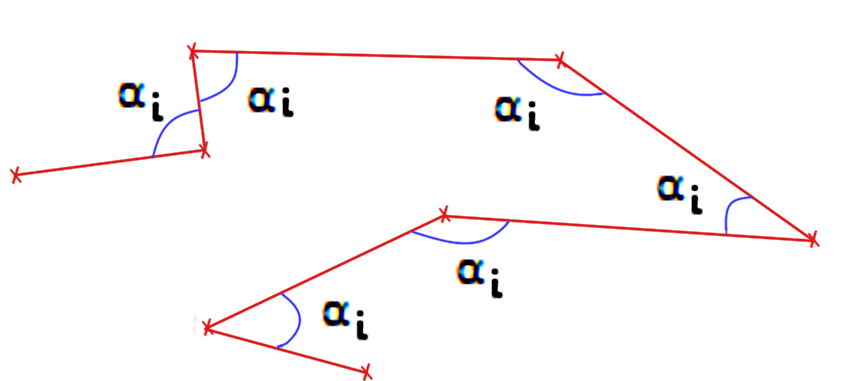
\includegraphics[width=\linewidth]{TrajectoirAlpha3.png}
%  \caption{extraction of the curve angle in the trajectory }\label{fig:trajectoirAlpha}
%  \endminipage\hfill
%\end{figure}

 \begin{mfigures}[!]{optimisation of the path plannig}{fig:trajectoirAlpha} \centering
\mfigure{width=.4\linewidth}{img/TrajectoirAlpha3.png}{Extraction of the curve angle in the trajectory.}{subfig:trajectoirAlpha}
\end{mfigures} 

To estimate the complexity of the trajectory two indicator are used in order to evaluate properly the distance of the trajectory and the complexity in term of curve for the UAV evolving in the 3D space.
Therefore the complexity of trajectory are computed as follow: 
\begin{equation}\label{Eq:trajectory}
\mbox{Trajectory complexity}=\frac{ \sum_{i=1}^{size(\alpha)} 180- \alpha_{i}  }{size(\alpha)}   
\end{equation}
Where $\alpha_i$ is a angle of curve in the trajectory as in figure \ref{fig:trajectoirAlpha}. \\
$Size(\alpha)$ is the number of curve in all the trajectory.\\

%%%%%%%%%%%%%%%%%%%
			\section{Experiment}
		\subsection{Comparison of the trajectory} \label{trajectoire path}
 
% \begin{figure}[t]
%  \centering
%   \subfigure[Path planing using the pattern method]{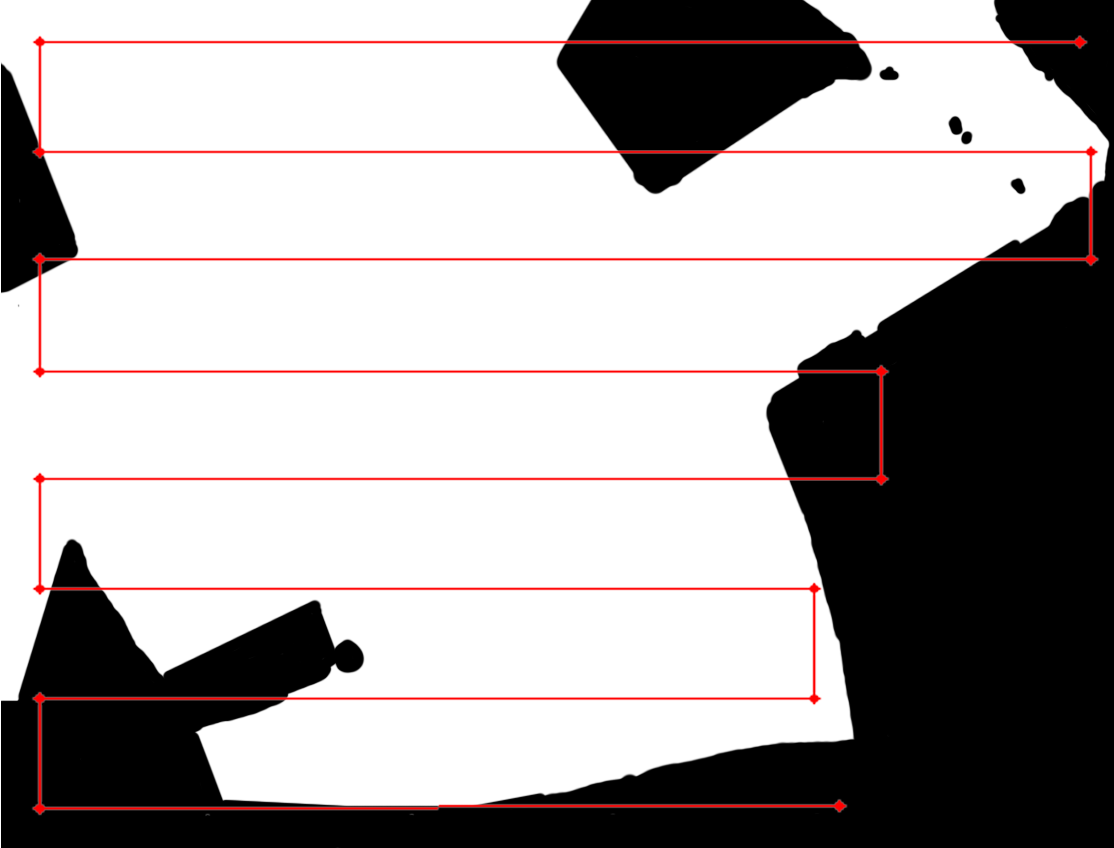
\includegraphics[width=0.49\textwidth]{calvisson2maskPath.png}}
%   \hfill
%   \subfigure[110 waypoints for 94.86\% of coverage]{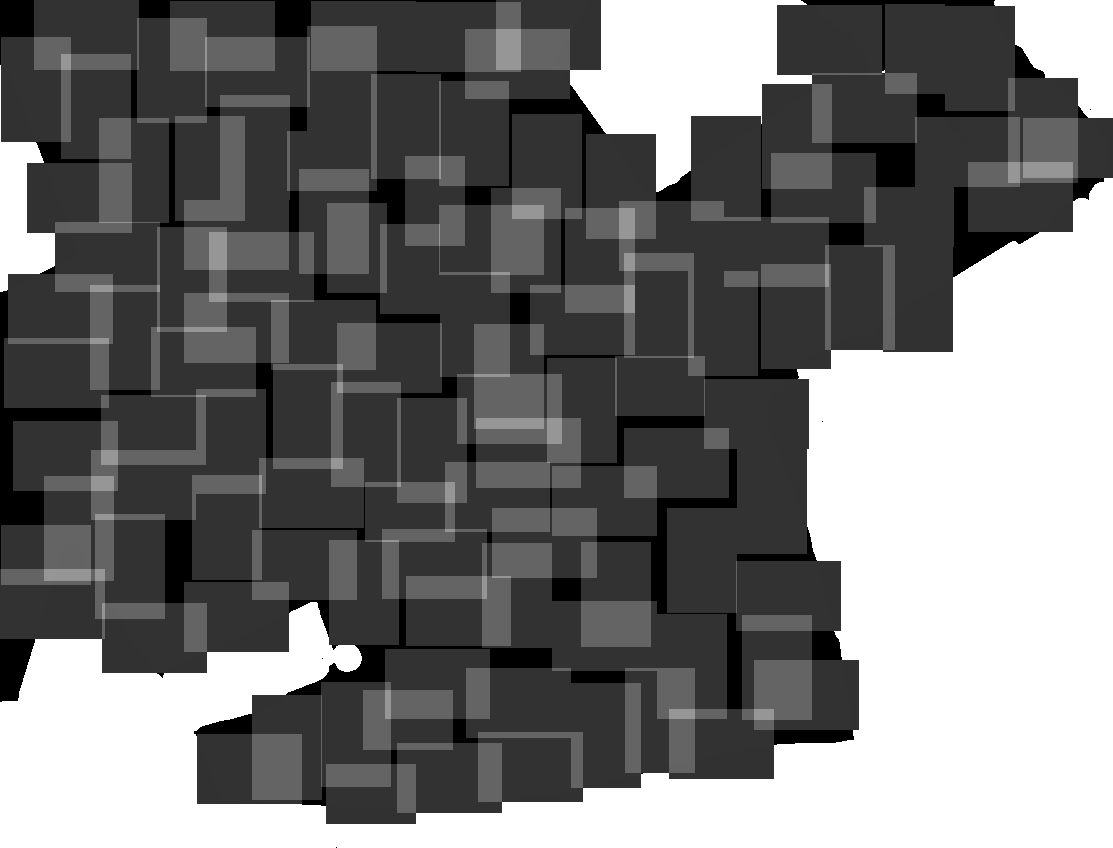
\includegraphics[width=0.49\textwidth]{zcalvisson2result1cout_94_862284_gen_3634_Ncam_110.png}}
%  
%  \subfigure[Path with 110 waypoints for 94.86\%  ]{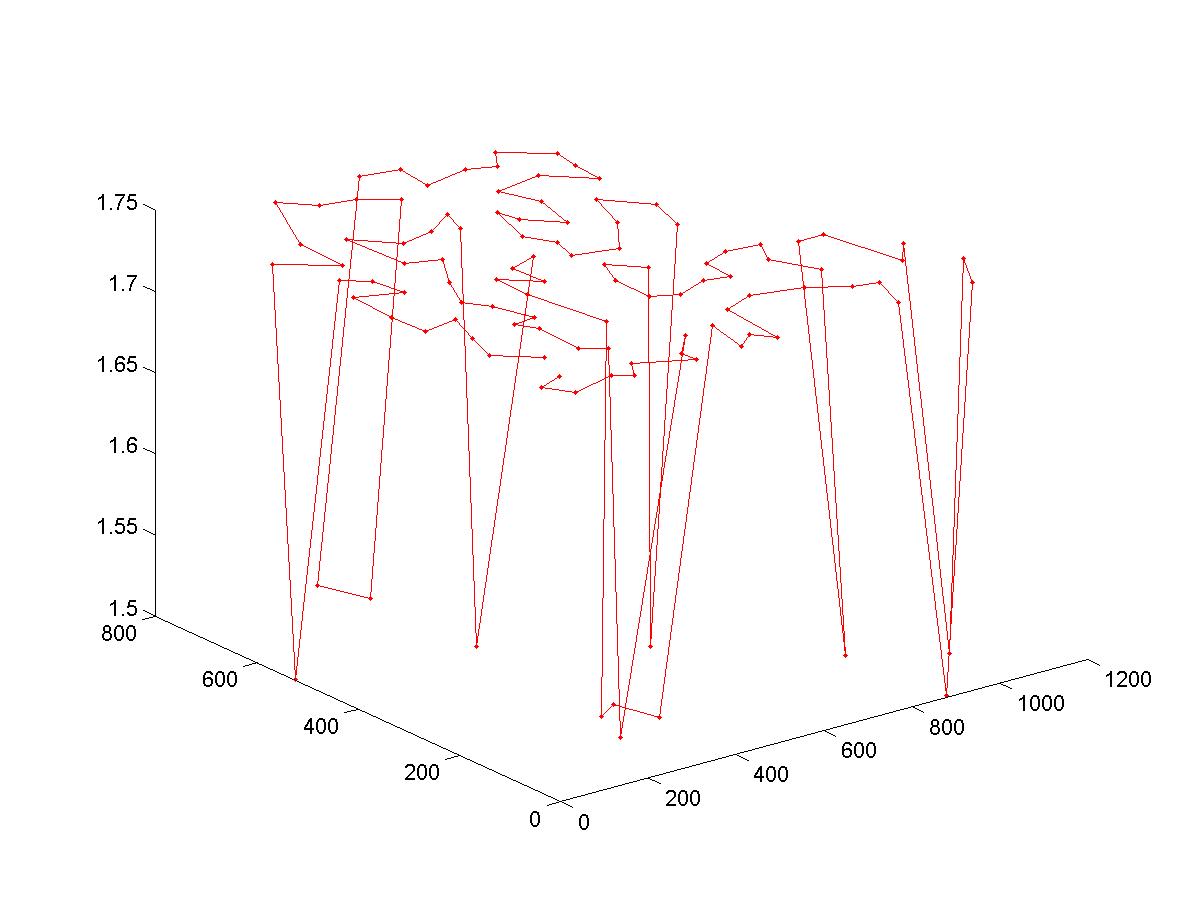
\includegraphics[width=0.85\textwidth]{zGAevolvTurnComplexCross_919Mut_001pop100cout_94_862284_gen_3634_Ncam_110Sorted.png}}
%  \caption{Room Coverage}\label{fig:trajectoryPath} 
%\end{figure}

 \begin{mfigures}[!]{optimisation of the path planing}{fig:trajectoryPath} \centering
\mfigure{width=.4\linewidth}{img/calvisson2maskPath.png}{Path planing using the pattern method.}{subfig:Dijktra}
\hspace{1cm}
\mfigure{width=.4\linewidth}{img/zcalvisson2result1cout_94_862284_gen_3634_Ncam_110.png}{Path compute with Dijktra multi goal.}{subfig:GATSP}
\mfigure{width=.4\linewidth}{img/zGAevolvTurnComplexCross_919Mut_001pop100cout_94_862284_gen_3634_Ncam_110Sorted.png}{Room Coverage.}{subfig:GATSP}
\end{mfigures} 
  In order to compare the efficiency of the trajectory computation proposed in this article with a standard method using a adapted pattern to cover an area. The patterned method apply is based on several article as \cite{63*,66*,pattern155*}
%  [ CHAO, Haiyang, BAUMANN, Marc, JENSEN, Austin, et al. Band-reconfigurable multi-UAV-based cooperative remote sensing for real-time water management and distributed irrigation control. In : IFAC World Congress, Seoul, Korea. 2008. \\]
%  [ ZHANG, Houxiang, ZHANG, Jianwei, et ZONG, Guanghua. Cleaning Trajectory Evaluation of a Wall Cleaning Robot Based on Synthesis Standards. In : Computational Engineering in Systems Applications, IMACS Multiconference on. IEEE, 2006. p. 1695-1700. \\]
%  [GALCERAN, Enric et CARRERAS, Marc. A survey on coverage path planning for robotics. Robotics and Autonomous Systems, 2013, vol. 61, no 12, p. 1258-1276.\\]. 
 %Predicate on the pattern method a path are compute on the area see fig ££££££££ calvison vide  £££££££££.
 The path proposed is establish on the area to cover and the camera field of view. The pattern is adapted depending then the shape of the area and the size of the camera projection in order to have a full coverage with the minimum of overlap. The final path using the pattern method as in figure \ref{fig:trajectoryPath}(a)
 \\In the other hand the solution proposed ( see figure \ref{fig:trajectoryPath}(b)) establish an path apparently more complex (see figure \ref{fig:trajectoryPath}(c)) using the third dimension with a coverage rate somewhat lower ( 94.86\% of coverage ).
 Although  the distance of the path  and the complexity trajectory based on  the equation \ref{Eq:trajectory} prove the efficiency of this method by a lower distance and a better complexity indicator as in table \ref{table:trajectory}.\\ 
 \begin{table}[t]
\begin{tabular}{|p{1.5cm}|p{1.8cm}|p{1.8cm}|p{1.8cm}|}
  \hline
   &Coverage rate & Path length (in px) &Trajectory complexity (eq:\ref{Eq:trajectory})  \\  \hline
  Pattern Method &  100\% & 9076 &90 \\ \hline
  Ours Method &  94.86\% & 8161 &69.81 \\ \hline
\end{tabular}
\caption{comparative table  of path distance and complexity.}\label{table:trajectory}
\end{table}
 
%  Dans cette partie on comapare des une methode  de calcule des trajectoire classique qui utilise des la repetition de paterne pour couvrire une zone.
%   l'avantage de la methode  utilisent des paternes et que l'on optien un taux de reconvrement beaucoup plus important qui  est de  100\% avec un taux de recouvremnt plus ou moin important. mais en contre partie l chemian parcourie et plus long, 200m contre 150m avec l'utilisation des algo génétique. concernant la complexité de la trajectoire  on s'appuit sur l'equation  

\subsection{Indore simulation} \label{experiment}
The simulated room is 30 $\times$ 28 m$^2$ which corresponds more or less to a large lecture hall or even an outdoor area. The areas in red (figure \ref{fig:final_room2} c)represents the zones which do not require coverage. Every camera can cover a 4 $\times$ 3 m$^2$  when $z$ is equal to one. The $z$ factor can be equal at $[0.5, 1, 1.5]$, and the cameras can turn  at 90$^{\circ}$. All of these parameters are taken into account in order to compute the waypoints and the GA was used but without any lock to the convergence. 
ROS is used to execute the path and send navigation commands to the robot.
% refer to : https://en.wikipedia.org/wiki/Screw_theory#Twist

These messages contain the linear and angular velocity values needed to control the robot's position and orientation. This process is to make the transition from simulation to real world UAV straightforward. The number of waypoints is set depending on the area covered by the cameras projection figure \ref{fig:cam_proj}. The trajectory built from these waypoints is done by sub-sampling the space between these 3D points coordinates.\\
In our experiments, V-REP \cite{Vrep} is used to simulate the hardware of the UAV and all its mounted sensors like camera which is the core sensor. 
% It was also used to build the room as explained in more details in the next subsection (\ref{experiment}). 
In order to ease the deployment of the algorithms on a real platform, we chose ROS \cite{ROS} as the implementation framework to command the simulated UAV.
 This experiment follow the pipeline showed in the figure \ref{fig:pipeline} with the two different optimization parts.\\
 
%  
%\begin{figure}[t]
%  \centering
%   \subfigure[Poses of every image captured in the room]{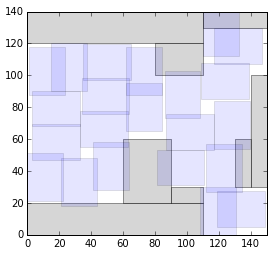
\includegraphics[width=0.45\textwidth]{room_python.PNG}}
%   \hfill
%   \subfigure[pose of every images with the path planning]{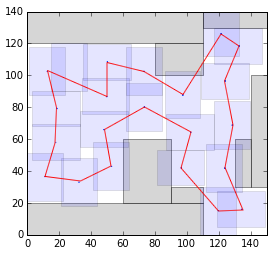
\includegraphics[width=0.45\textwidth]{room_pythonPath.png}}
%  
%  \subfigure[room in V-rep]{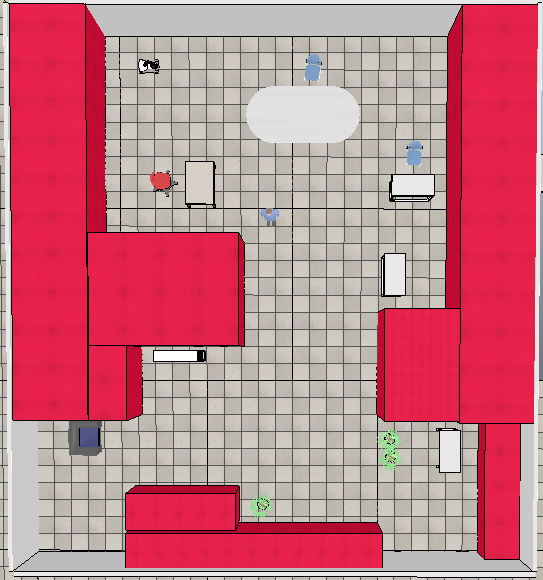
\includegraphics[width=0.45\textwidth]{room_full.png}}
%  \hfill
%  \subfigure[Room mosaicing]{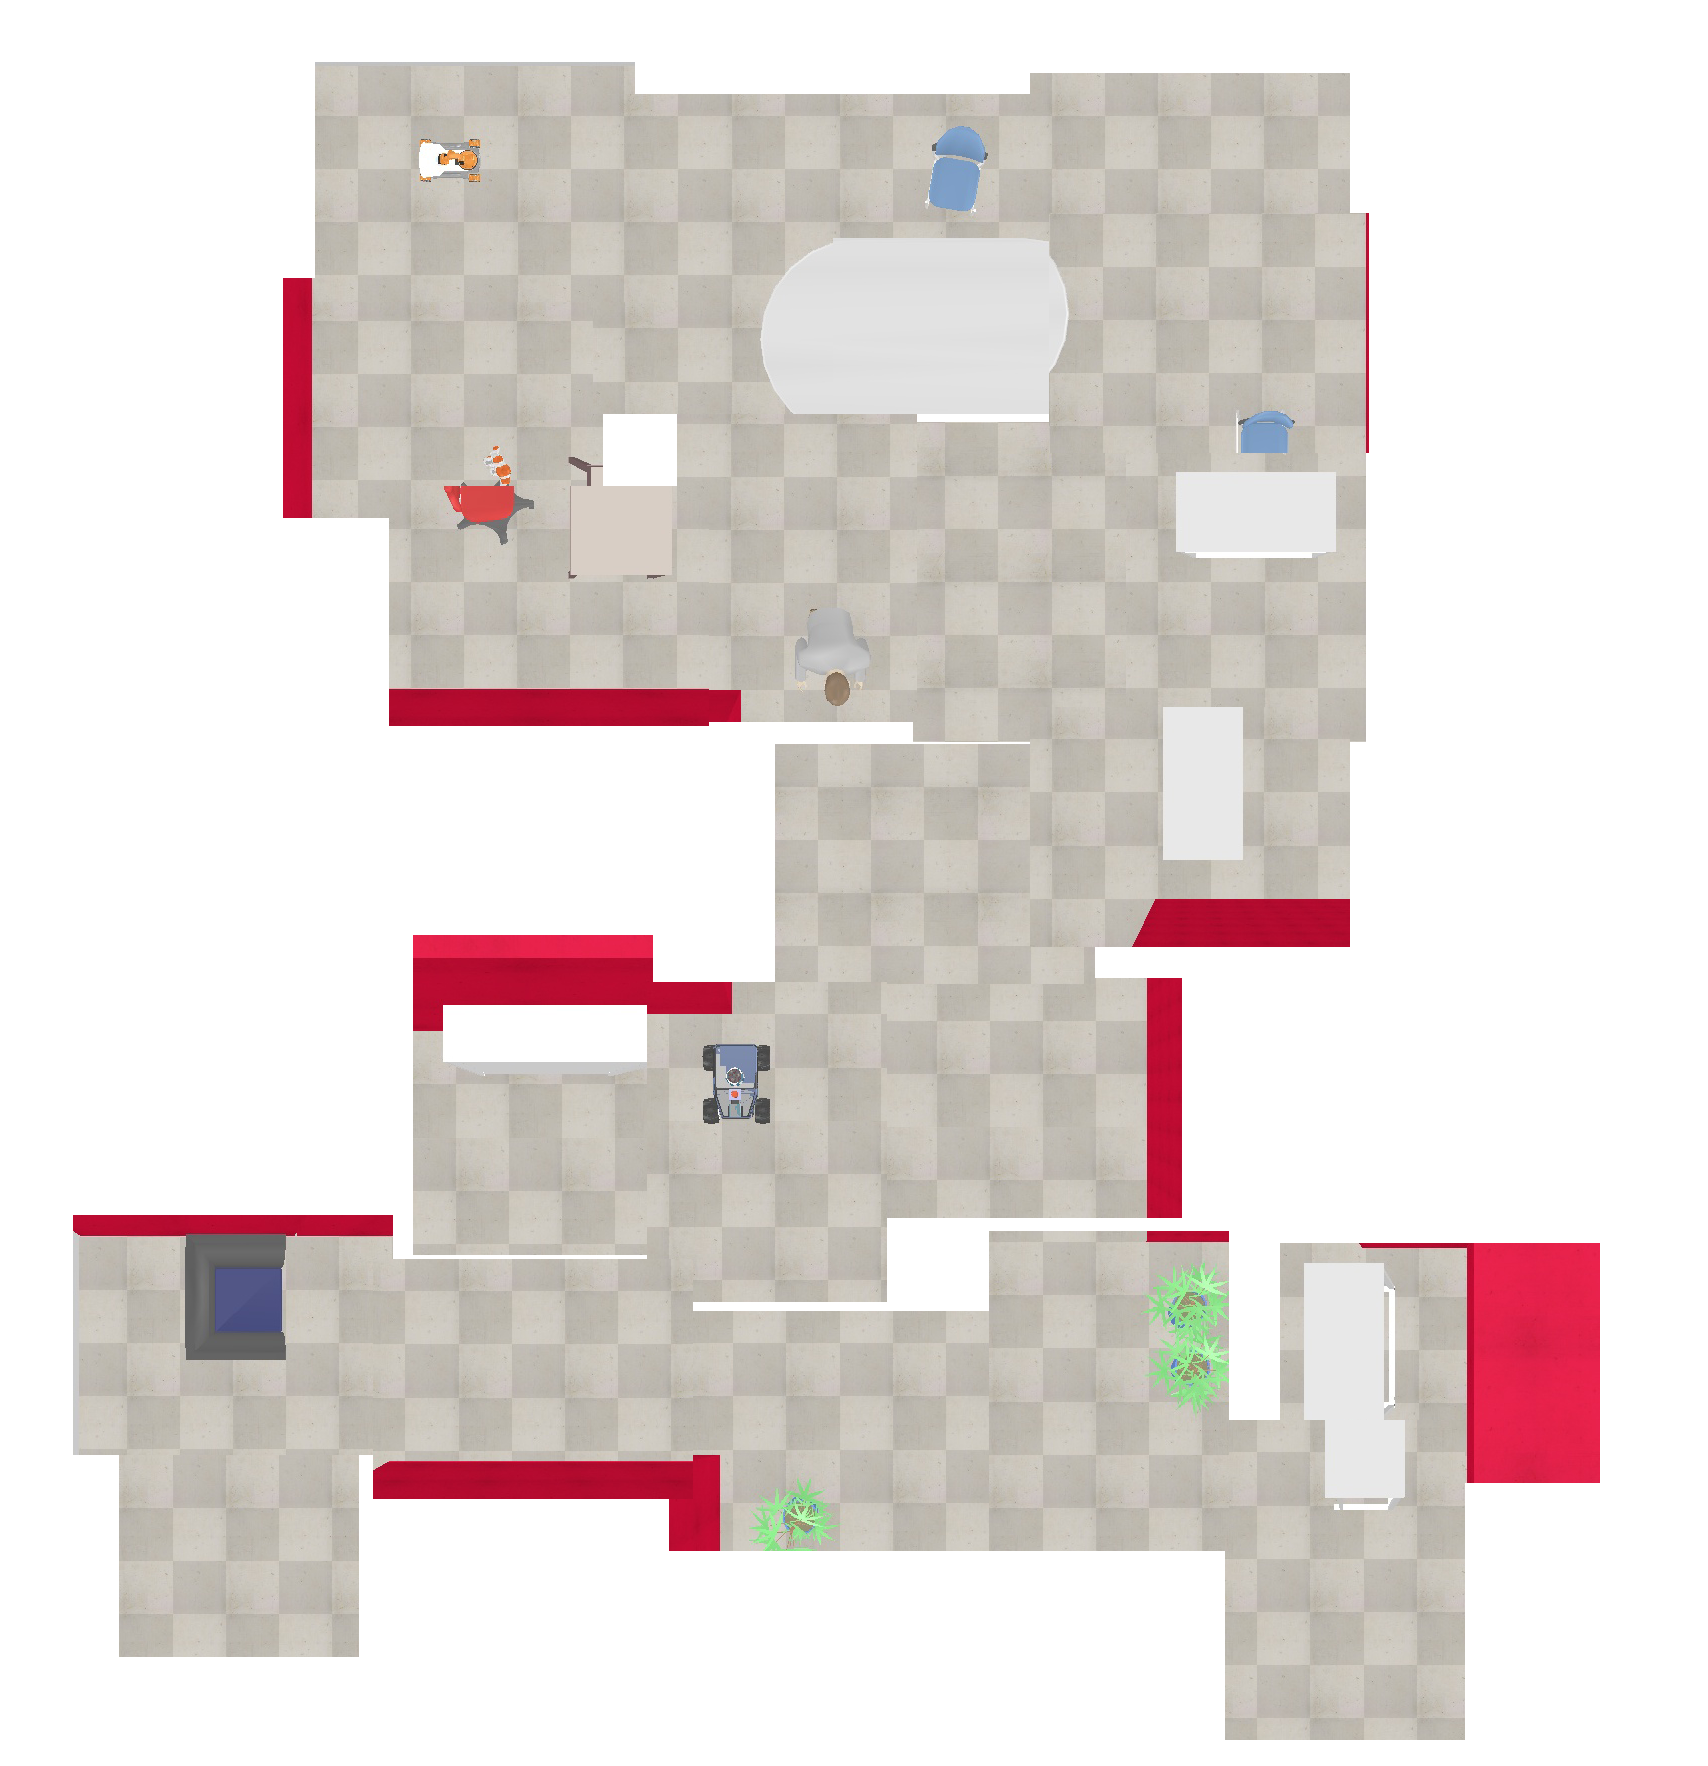
\includegraphics[width=0.45\textwidth]{mosaic2.png}}
%  \caption{Room Coverage}\label{fig:final_room2} 
%\end{figure}

 \begin{mfigures}[!]{optimisation of the path planing}{fig:final_room2} \centering
\mfigure{width=.4\linewidth}{img/room_python.PNG}{Poses of every image captured in the room}{subfig:RoomPy}
\hspace{1cm}
\mfigure{width=.4\linewidth}{img/room_pythonPath.png}{Pose of every images with the path planning}{subfig:PathPlanning}
\mfigure{width=.4\linewidth}{img/room_full.png}{Room in V-rep}{subfig:RoomVrep}
\mfigure{width=.4\linewidth}{img/mosaic2.png}{Room Coverage}{subfig:RoomCov}
\end{mfigures} 

 
 \subsubsection{Mosaicing }

The ortho-mosaiced output image composed by the captured
images should be very close to a complete top view of the area.
Mosaicing in our case is simply computed using the position coordinates of the known waypoint and stitch the images together to validate the optimum choice of the positions where the drone captured these images figure \ref{fig:final_room2}(d).

The coverage threshold rate is 90\% of the useful area in the room without taking the block parts into full consideration to cover.
 
 

\subsection{coverage outdoor}\label{coverageOutDoor}
 A much bigger area involves the increasing of the search space and the increasing of the complexity. 
In the following example figure \ref{subfig:satimgMask} the satellite images are used to define the area to control (in white)  by the UAV. \\
In order to cover the big area the solution can be to use a bigger focal or higher altitude to have a wide area covered at each waypoint, thus keep few waypoints to control the area. But the GA associate to the adapted cost function allows on the example figure \ref{subfig:satimgcoverage} much more waypoints to be placed and optimized, compared to the literature for example, in \cite{c10,c11}. In the figure \ref{subfig:satimgcoverage} and \ref{subfig:satimgNoncover} the area is covered by 110 waypoints for 98.26$\%$ of coverage and the convergence are achieved after 170501 generations.\\



%\begin{figure}[t]
%  \centering
%  \hspace*{\fill}
%  \subfigure[]{\label{subfig:satimg+mask}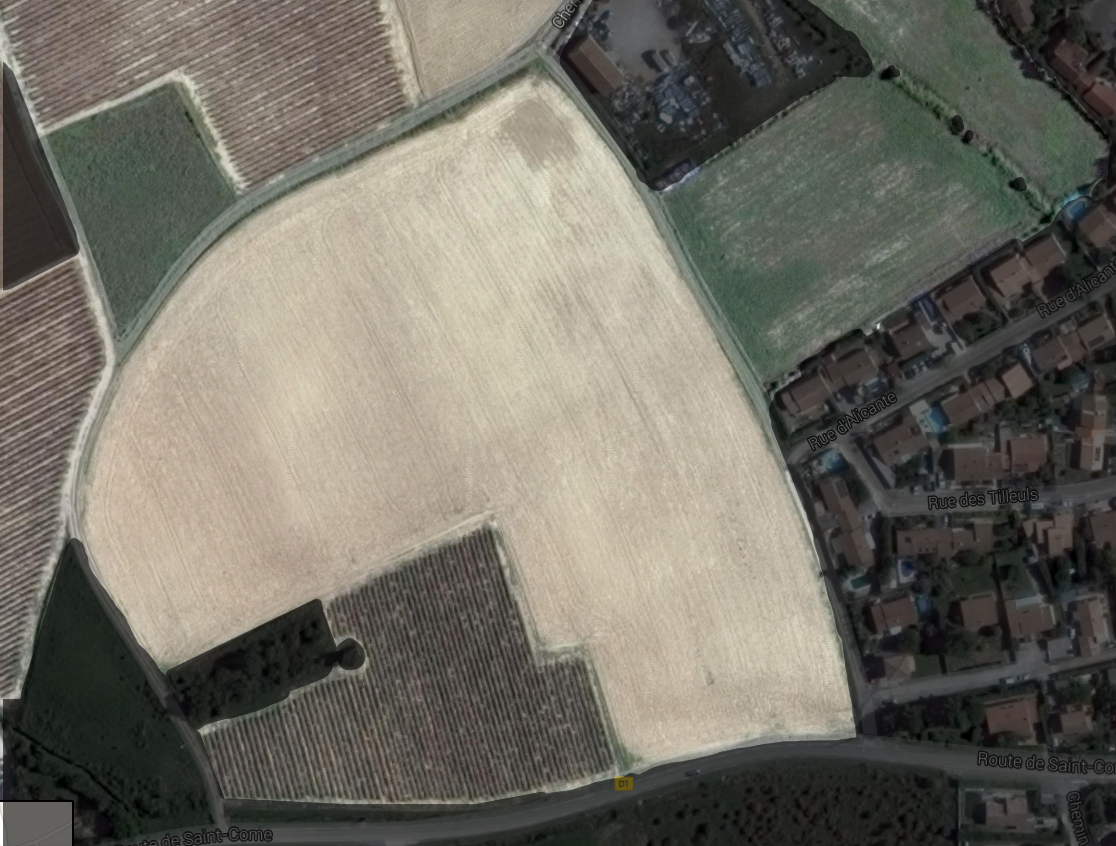
\includegraphics[width=0.48\linewidth]{calvisson2+mask.png}} \hfill
%  \subfigure[]{\label{subfig:satimgMask}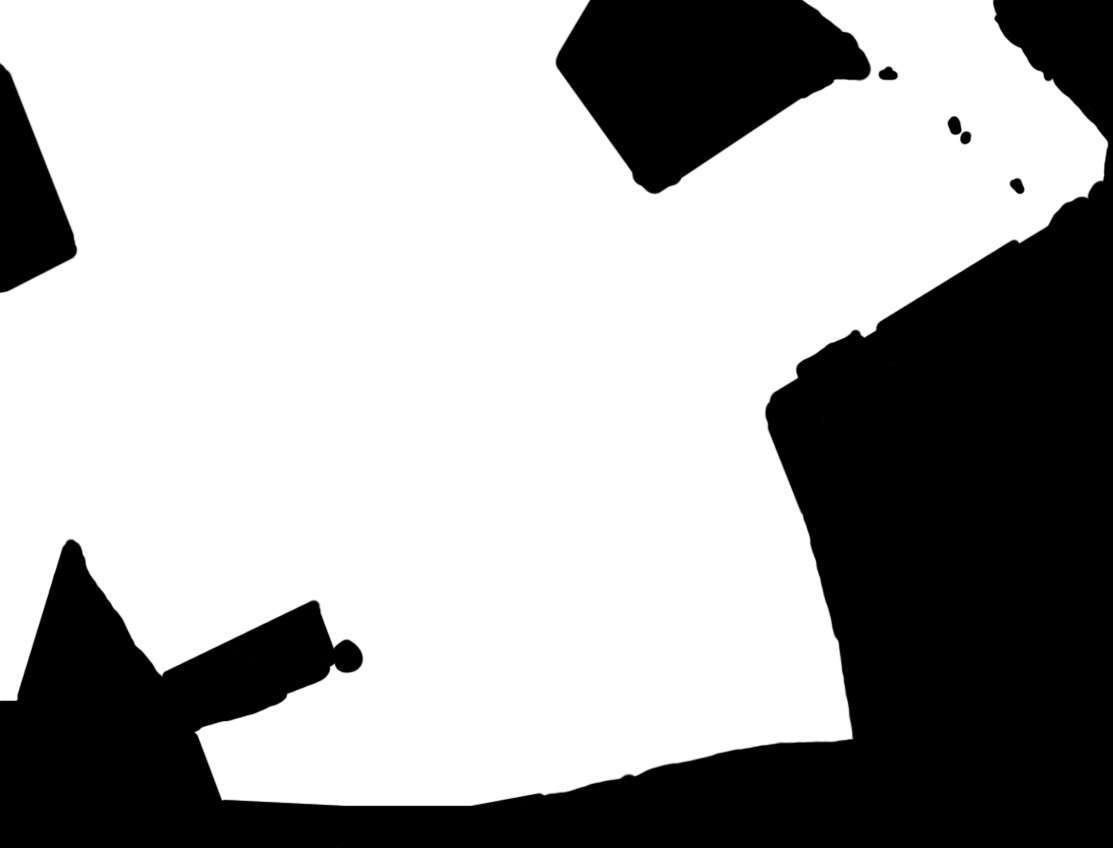
\includegraphics[width=0.49\linewidth]{calvisson2mask.png}}
%  \hspace*{\fill}
%  \\
%   \hspace*{\fill}
%  \subfigure[]{\label{subfig:satimgcoverage}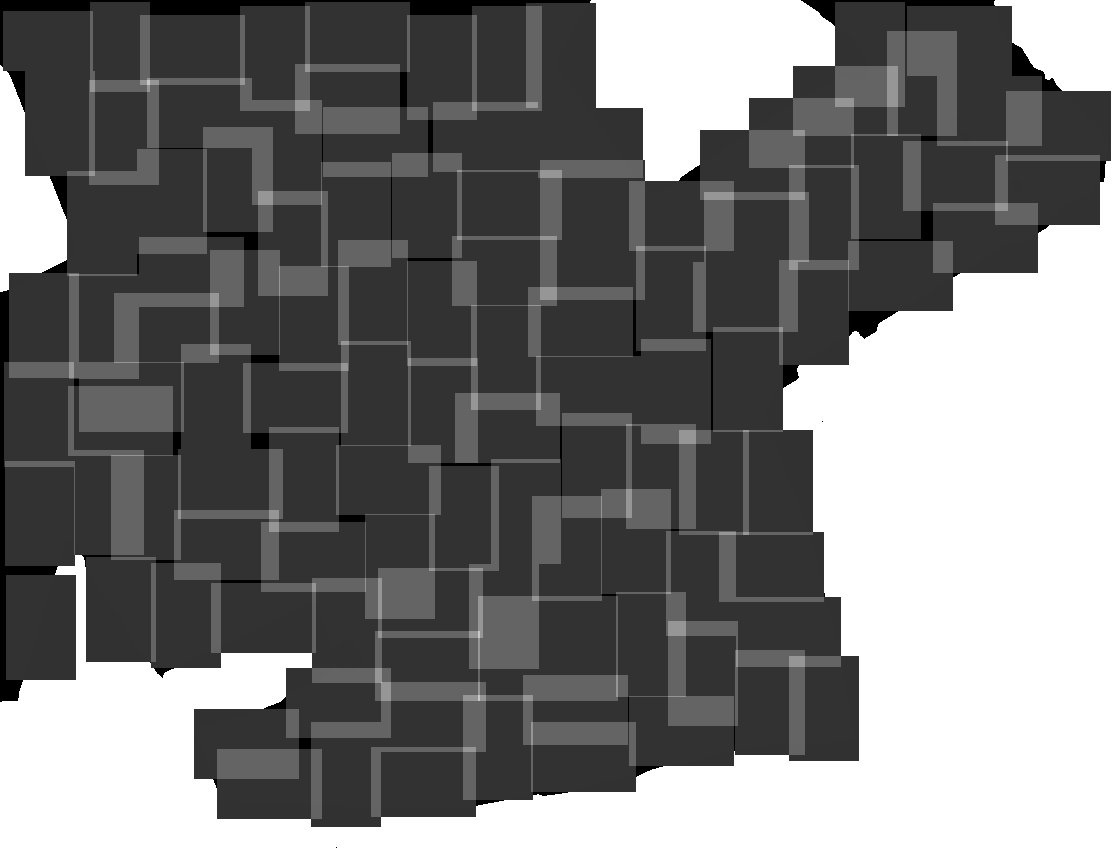
\includegraphics[width=0.80\linewidth]{zcalvisson2result1cout_98_260375_gen_170501_Ncam_110.png}}
%  \hspace*{\fill}
%  \hspace*{\fill}
%  \subfigure[]{\label{subfig:satimgNoncover}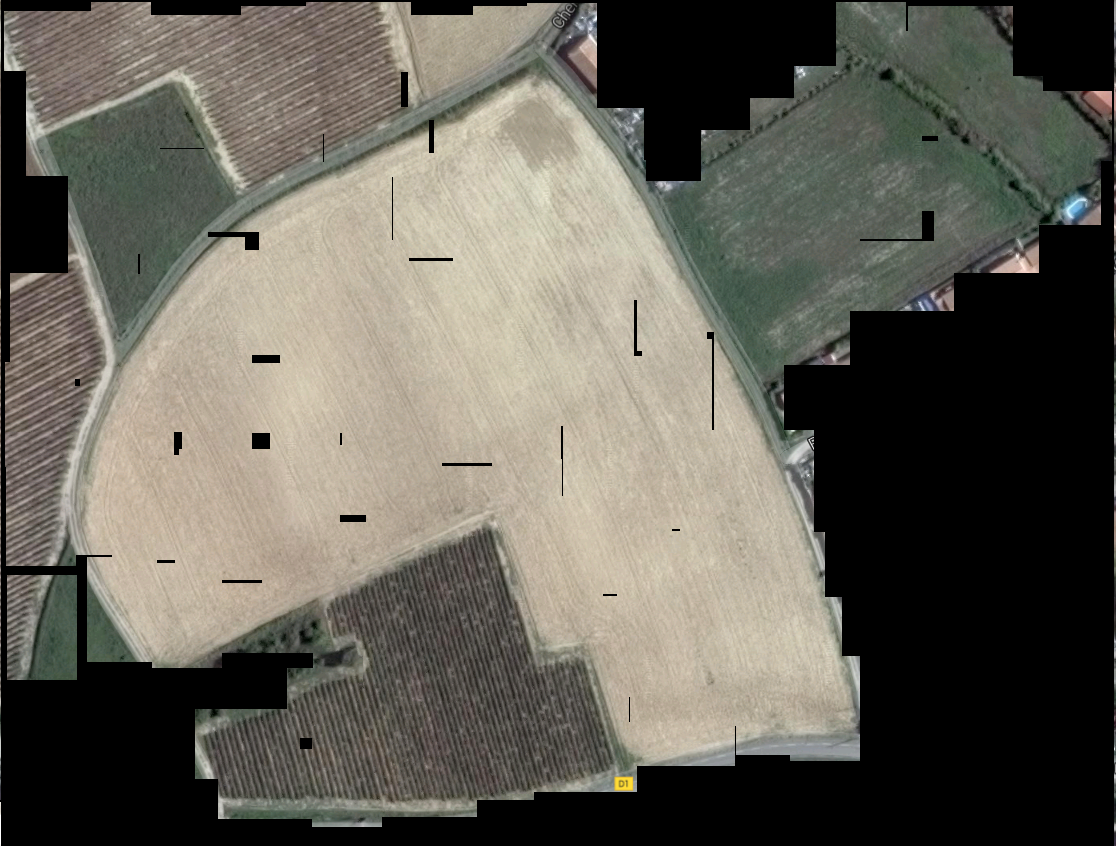
\includegraphics[width=.8\linewidth]{calvisson3cover.png}} \hfill
%  \hspace*{\fill}
%  \caption{ Optimization of the waypoint pose with a big outside area: (a) is the area to cover take form a satellite images,(b) is a mask of the area to cover, (c) is a result of the coverage with the waypoint position, (d) is the representation of the black hole.}
%  \label{fig:Rooms_shapes}
%\end{figure}
\subsubsection{Vast and complex outdoor}\label{sec:fey_map_CPPP}
\subsubsection{Biggest map with numerous waypoints}

\section{Use GA with non splitting in sub problem }
		\subsection{Explosion  de la complexité }
		\subsection{Result }
Use GA with non splitting in sub problem
			Explosion  de la complexité 
			Result 

%%%%%%%%%%%%%%%%%%%%%%%%%%%%%%%%%%%%%%%%%%%%%%%%%%%%



